\documentclass{article}
\usepackage[utf8]{inputenc}
\usepackage{graphicx}
\usepackage{epstopdf}
\usepackage{float}
\usepackage[margin=1.25in]{geometry}
\usepackage{amsmath}
\usepackage{amssymb}
\usepackage{color} 
\usepackage{fancyvrb} 
\newcommand{\Vout}{{$V_{out}$}}
\newcommand{\Vb}{{$V_{b}$}}
\newcommand{\Vcm}{{$V_{cm}$}}
\newcommand{\Vdm}{{$V_{dm}$}}
\newcommand{\Vtwo}{{$V_{2}$}}
\newcommand{\Vone}{{$V_{1}$}}
\newcommand{\Itwo}{{$I_{2}$}}
\newcommand{\Ione}{{$I_{1}$}}
\newcommand{\Vdd}{{$V_{dd}$}}
\newcommand{\Iout}{{$I_{out}$}}
\newcommand{\Vin}{{$V_{in}$}}
\newcommand{\Gm}{{$G_{m}$}}
\newcommand{\Idm}{{$I_{dm}$}}
\newcommand{\Icm}{{$I_{cm}$}}
\newcommand{\Ib}{{$I_{b}$}}
\newcommand{\nMOS}{{\textit{n}MOS }}
\newcommand{\pMOS}{{\textit{p}MOS }}
\newcommand{\Mone}{{$M_{1}$}}
\newcommand{\Mtwo}{{$M_{2}$}}
\newcommand{\Mthree}{{$M_{3}$}}
\newcommand{\Mfour}{{$M_{4}$}}
\newcommand{\Mb}{{$M_{b}$}}
\newcommand{\Adm}{{$A_{dm}$}}
\newcommand{\Rout}{{$R_{out}$}}
\newcommand{\Ro}{{$R_{o}$}}
\title{Circuits Lab 8}
\author{Cory Dolphin and Noam Rubin}
\date{\today}

\begin{document}

\maketitle

\begin{figure}[H]
\centering
\includegraphics[width=0.6\linewidth]{../Figures/Lab8Schematic}
\caption{A schematic of the differential amplifier used in this lab, with some extra voltages and currents annotated for the purpose of analysis.}
\label{fig:lab8schem}
\end{figure}


\section*{Experiment 1}
We began by building a simple differential amplifier from an \nMOS differential pair and a \pMOS current mirror. We set the bias transistor just at threshold by applying a bias voltage of $V_B=0.6V$ We connected both inputs together such that the differential mode voltage was zero, and swept the common mode voltage from $+5V$ to $0V$, measuring the output voltage, \Vout. 
A plot of \Vout as a function of \Vcm can be seen below in Figure \ref{fig:exp1p1}. For values of \Vcm greater than the bias voltage, $0.6V$, \Vout appears to change very little with large changes in \Vcm.  We determined the common-mode gain of the amplifier by applying a linear fit to the data. The linear fit found had a slope $-0.202$, thus from our data, we experimentally found $A_{cm} = -0.202$. Notably, the output voltage appeared to stabilize at approximately $4.3V$.
Though we expected a negative common-mode gain on the order of a few percent, our gain is larger than expected, on the order of a tens of percents, instead of percents. This is likely caused by transistor mismatch.

\begin{figure}[H]
\centering
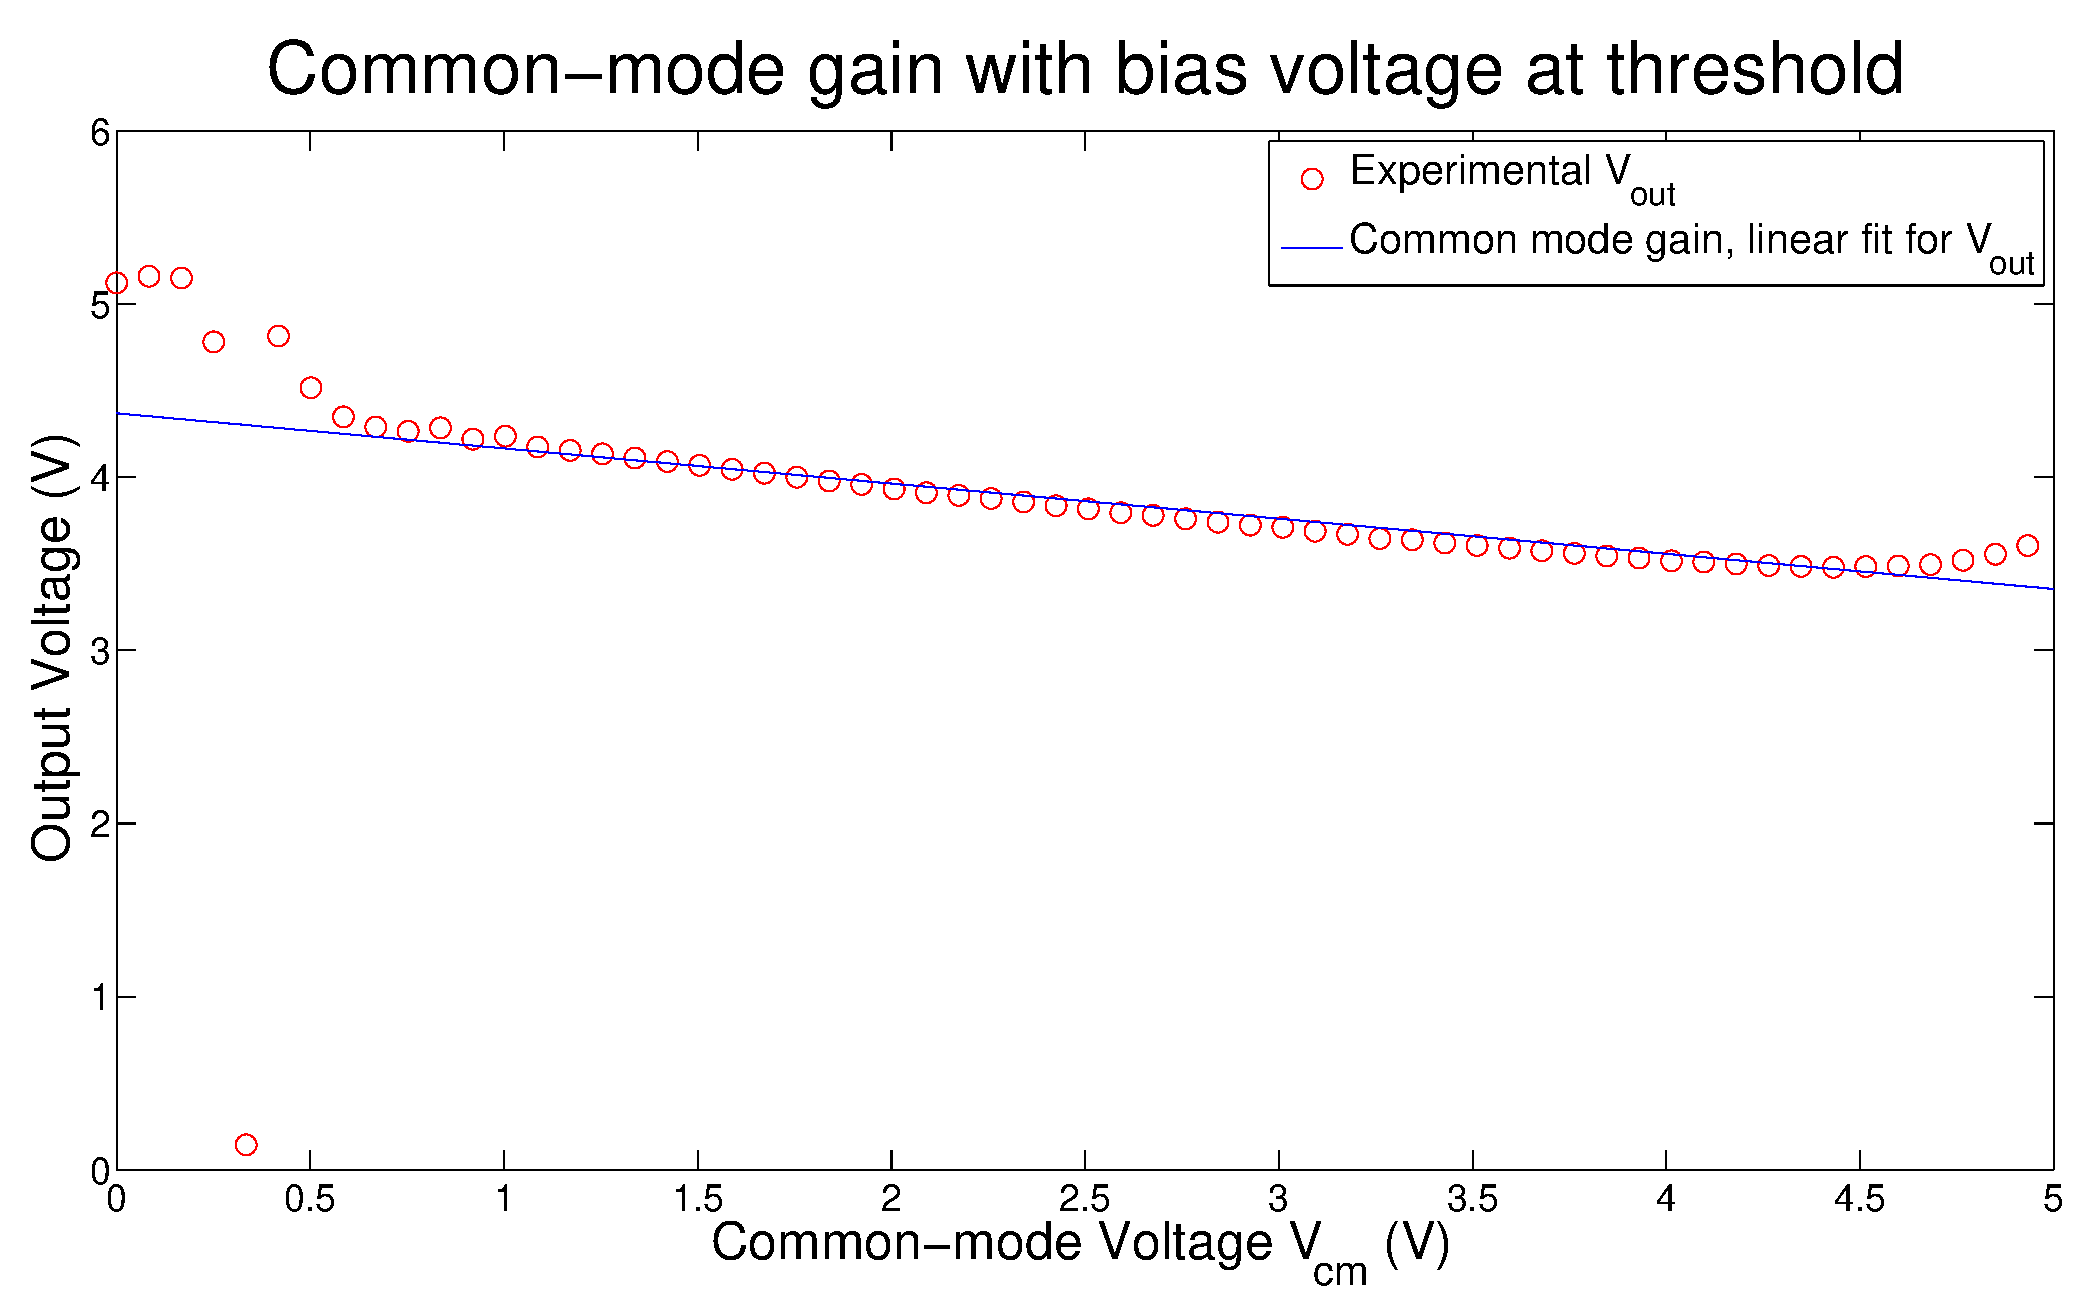
\includegraphics[width=\linewidth]{../Figures/Exp1P1.eps}
\caption{For values of \Vcm greater than the bias voltage, $0.6V$, \Vout appears to change very little with large changes in \Vcm.  We determined the common-mode gain of the amplifier by applying a linear fit to the data. The linear fit found had a slope $-0.202$.}
\label{fig:exp1p1}
\end{figure}

We then connected \Vtwo to a constant voltage source and sweep \Vone from one $+5V$ to $0V$, measuring \Vout for \Vtwo set to three different voltages, $2V$, $3V$ and $4V$.

The voltage transfer characteristic for these experiments, shown in Figure \ref{fig:exp1p2} show three major regions of operation: one in which \Vout increases linearly with a small slope relative to \Vone, when \Vone is less than \Vtwo; another in which \Vout rapidly increases to the positive rail over a small voltage range, when \Vone is slightly greater than \Vtwo; and a third, in which \Vout is pinned at the $+5V$ rail.


\begin{figure}[H]
\centering
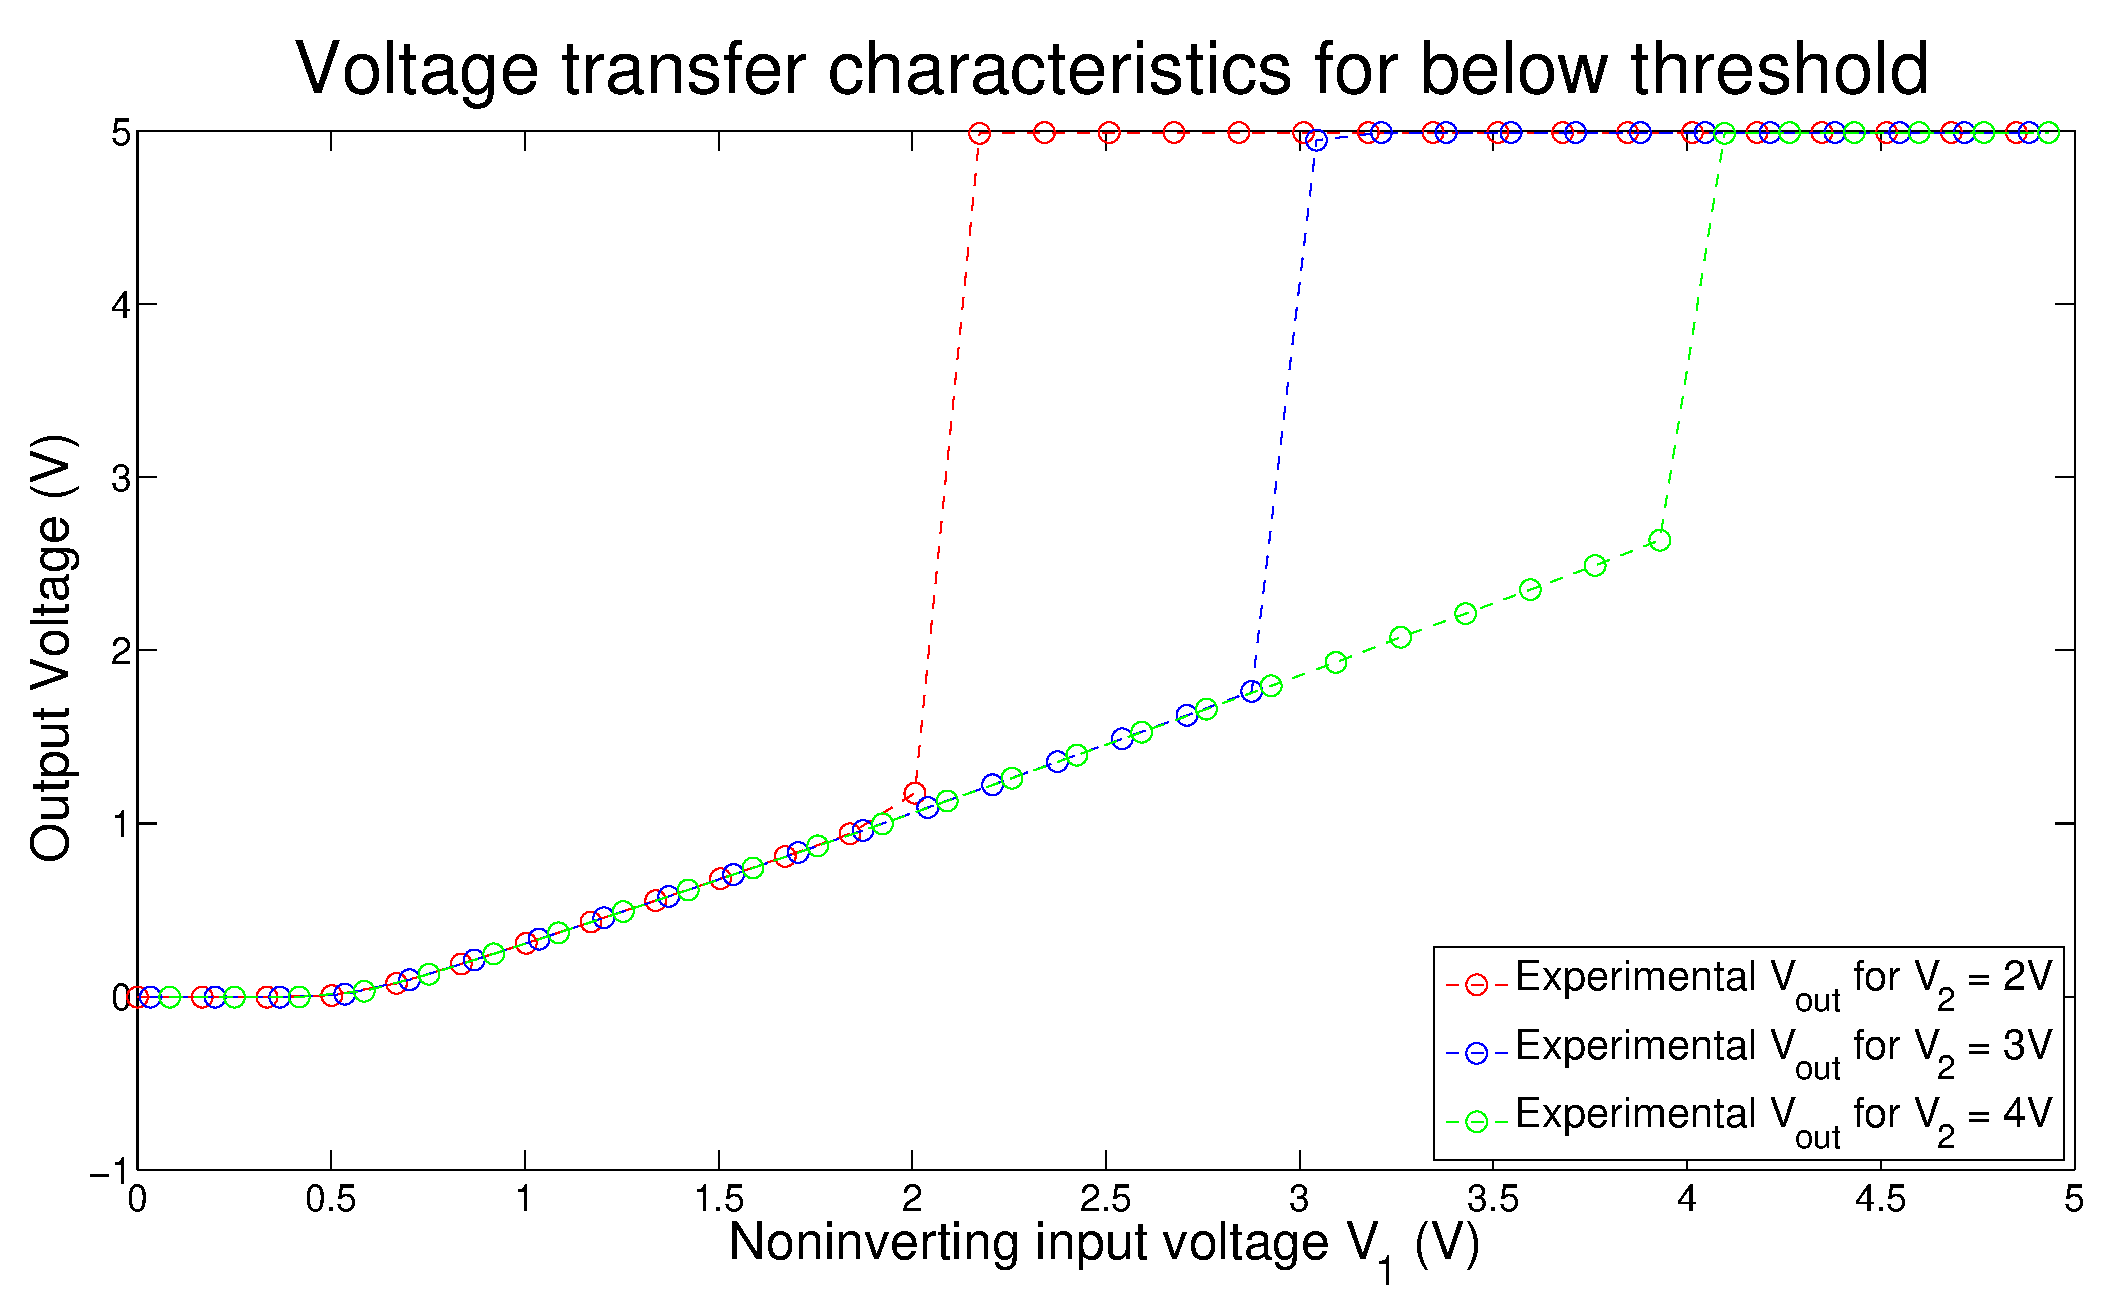
\includegraphics[width=\linewidth]{../Figures/Exp1P2.eps}
\caption{Note that the three series are similar in shape, with the point of inflection equaling the second input voltage for each series.}
\label{fig:exp1p2}
\end{figure}


Repeating the experiment with the bias transistor in strong inversion, with $V_b = 1.5V$, we found a similar pattern to the previous experiment, though the time-scale seemed to be extended.

In the case of the common-mode gain, we found that \Vout ultimately achieved a voltage of roughly $3.8V$, roughly $0.5V$ less than in the weak inversion case. Further, \Vout changed even less relative to \Vcm when \Vcm was greater than \Vb. With the bias transistor strongly inverted, we found a common-mode gain of $-0.039$, a magnitude more similar to the value expected. Meanwhile, for common-mode voltages less than \Vb, \Vout changed far more rapidly.

\begin{figure}[H]
\centering
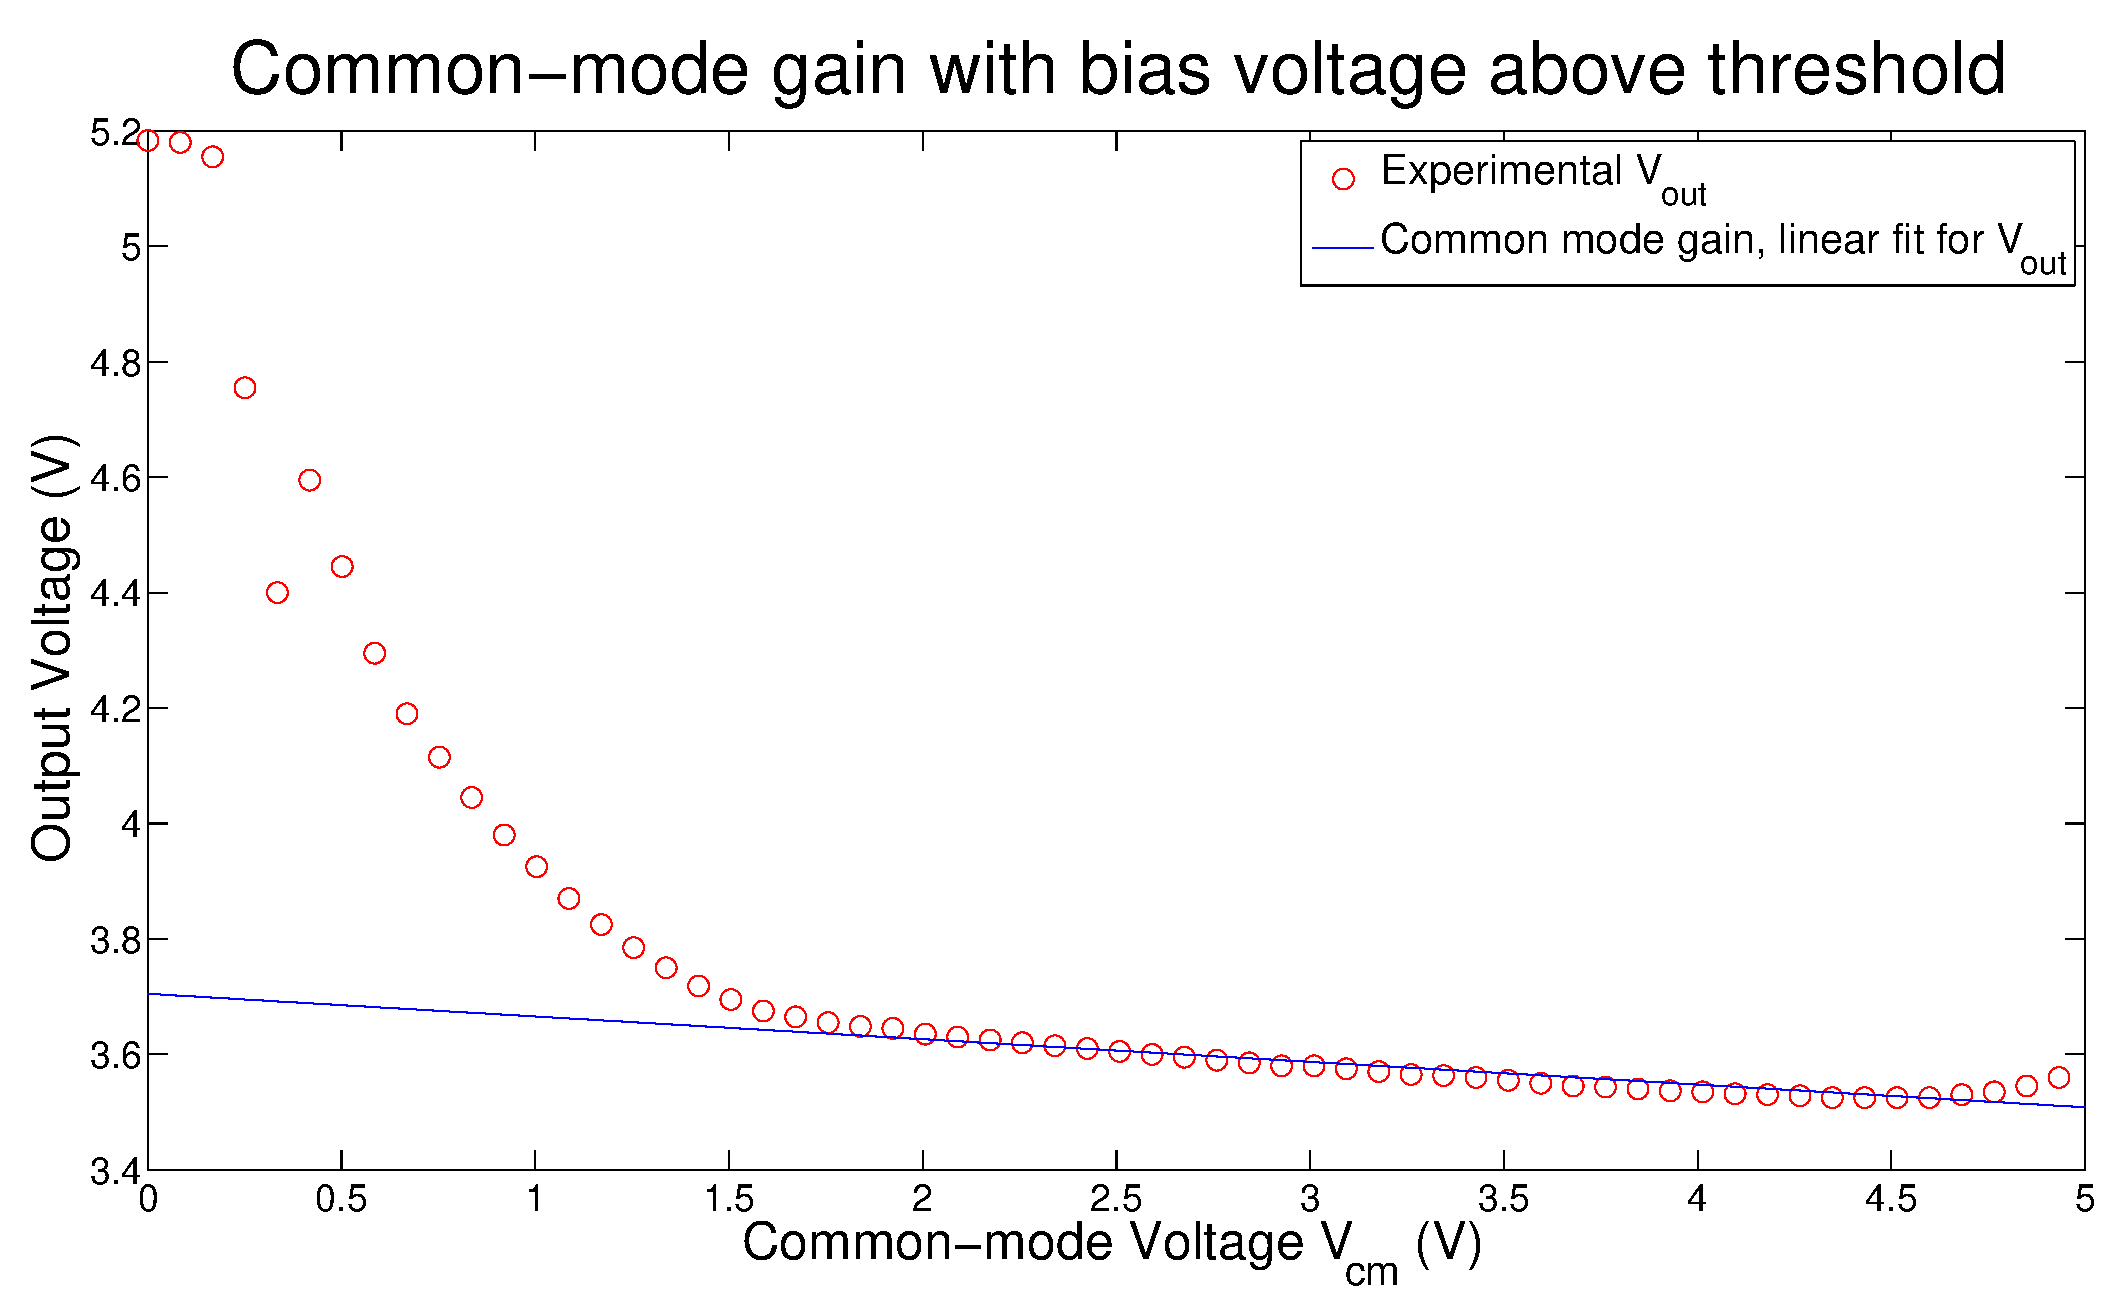
\includegraphics[width=\linewidth]{../Figures/Exp1P4.eps}
\caption{Something descriptive..}
\label{fig:exp1p4}
\end{figure}

When sweeping \Vdm through a range of values, we found that a similar relationship held, three major regions were found on the voltage transfer characteristic shown in Figure \ref{fig:exp1p3}:one in which \Vout increases linearly with a small slope relative to \Vone, when \Vone is less than \Vtwo; another in which \Vout rapidly increases to the positive rail over a small voltage range, when \Vone is slightly greater than \Vtwo; and a third, in which \Vout is pinned at the $+5V$ rail.
One major difference between the behavior with the bias transistor in strong inversion was the rate at which \Vout changed when \Vone increased just past \Vtwo; the output voltage approached the $+5V$ rail more slowly than in the weak inversion case, and appeared to somewhat smooth the discontinuities found in the previous case, linking the three regions with a more sigmoidal shape.

\begin{figure}[H]
\centering
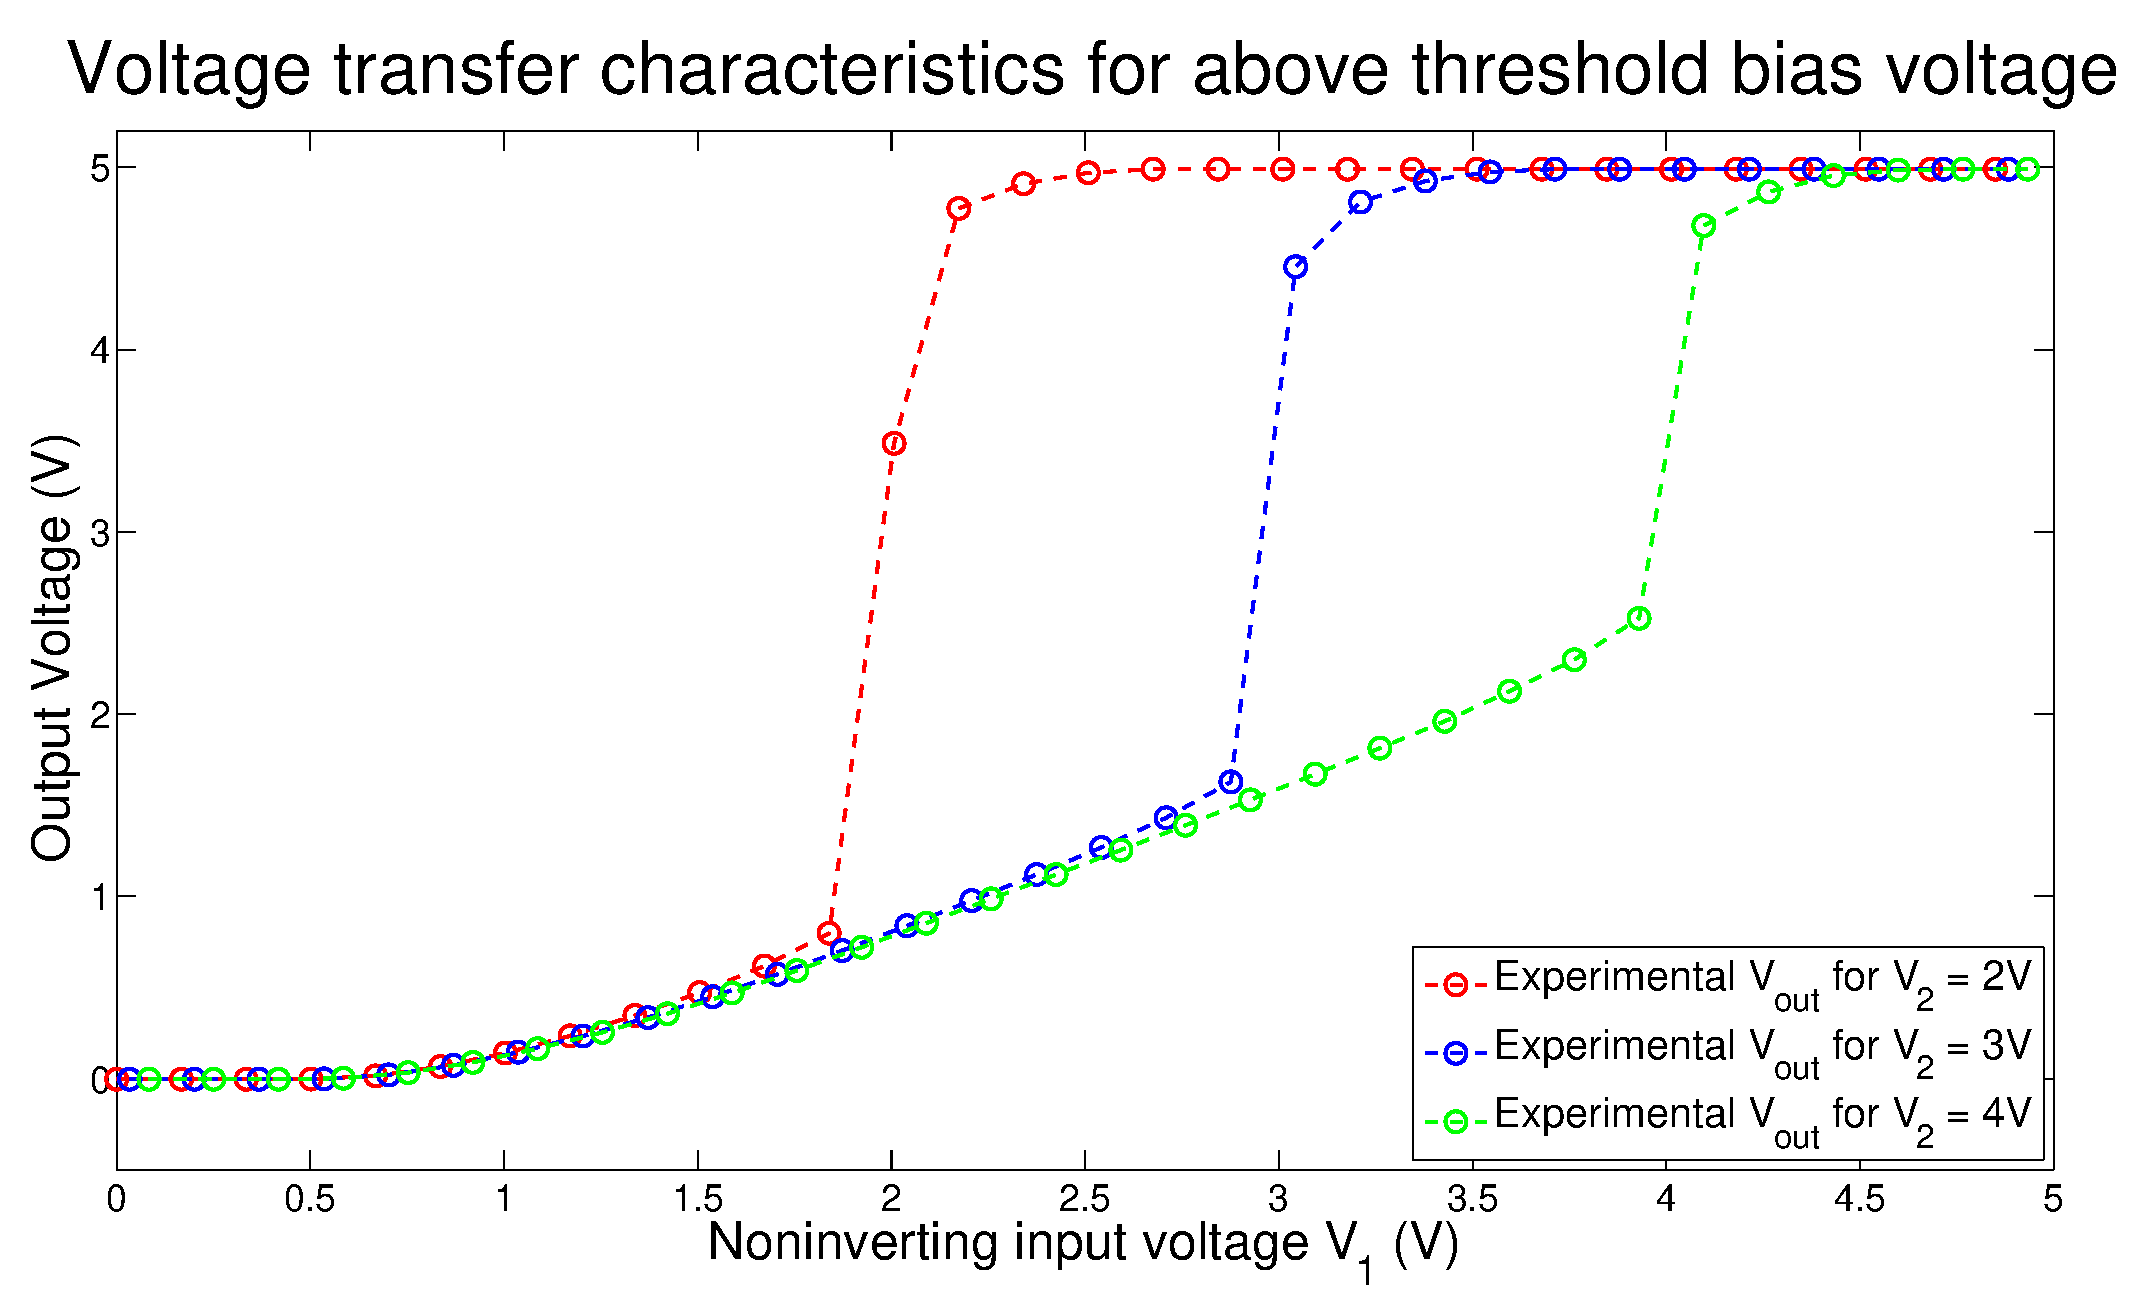
\includegraphics[width=\linewidth]{../Figures/Exp1P3.eps}
\caption{Note that the three series are similar in shape, with the point of inflection equaling the second input voltage for each series.}
\label{fig:exp1p3}
\end{figure}


The behavior of the circuit does not seem to differ substantially when biased in strong inversion, when compared to that which it exhibits in weak inversion. The major difference is the somewhat diluted affect of $V_{dm}$, that is to say, when in strong inversion, larger swings in \Vdm were necessary to produce similar changes in \Vout. This can be seen in the comparison of Figure \ref{fig:exp1p4} and Figure \ref{fig:exp1p2}, where the abrupt discontinuities seen in weak inversion are smoothed out in strong inversion, as can be seen by the rounding of the sharp angles.


\section*{Experiment 2}

We then studied the incremental properties of the differential amplifier, most importantly the differential-mode voltage gain, \Adm. We define

\begin{equation}
A_{dm} = \frac{\partial V_{out}}{\partial V_{dm}} = \frac{\partial V_{out} }{\partial I_{out} } \cdot \frac{\partial I_{out}}{\partial V_{dm}}
\label{eq:adm}
\end{equation}

We can estimate \Adm for this circuit in two ways: the first is to measure \Vout as a function of \Vdm, and extracting the slope for small values of \Vdm. We can also collect curves for \Vout as a function of \Iout and \Iout as a function of \Vdm, and then multiply the linear region of those plots together in order to extract a value for \Adm.

\begin{figure}[H]
\centering
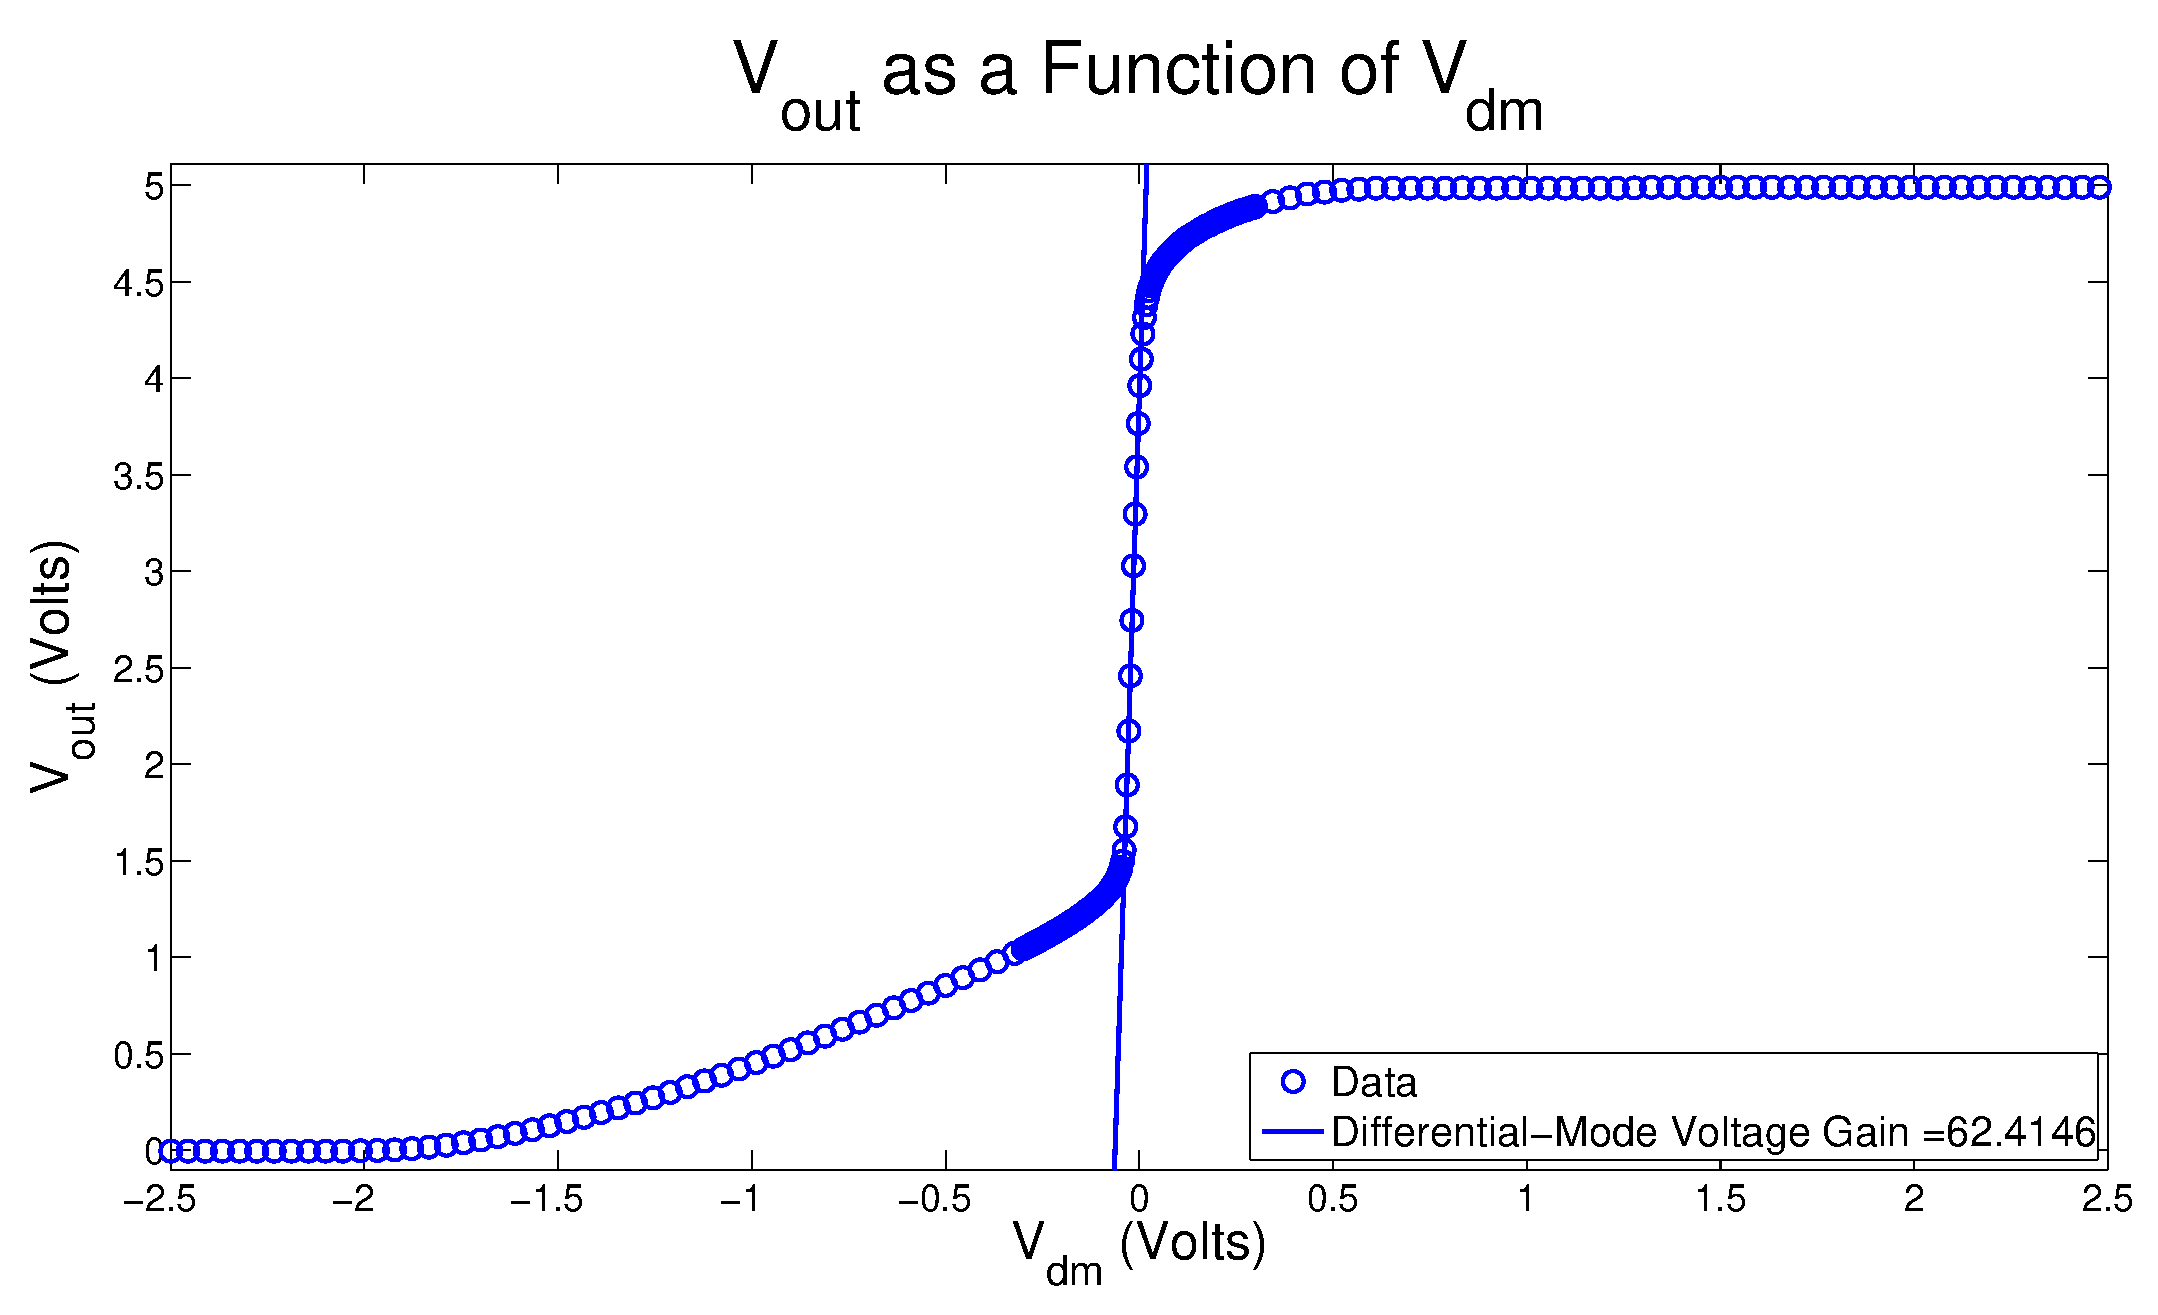
\includegraphics[width=\linewidth]{../Figures/Exp2P1.eps}
\caption{\Vout as a function of \Vdm. The interesting region in this graph is the near-vertical region around $|V_{out}| < 0.05 V$, as the slope of this region can be interpreted as \Adm, the differential mode voltage gain. From this plot we extracted an \Adm value of 62.4146.}
\label{fig:exp2p1}
\end{figure}

We first measured \Vout as we help \Vcm at 1.2 V and swept \Vdm from -0.5 V to 0.5 V. We plotted \Vout as a functions of \Vdm, as seen in figure \ref{fig:exp2p1}. In order to get a large number of points in the high-gain region, we collected data at different densities along \Vdm.

\begin{figure}[H]
\centering
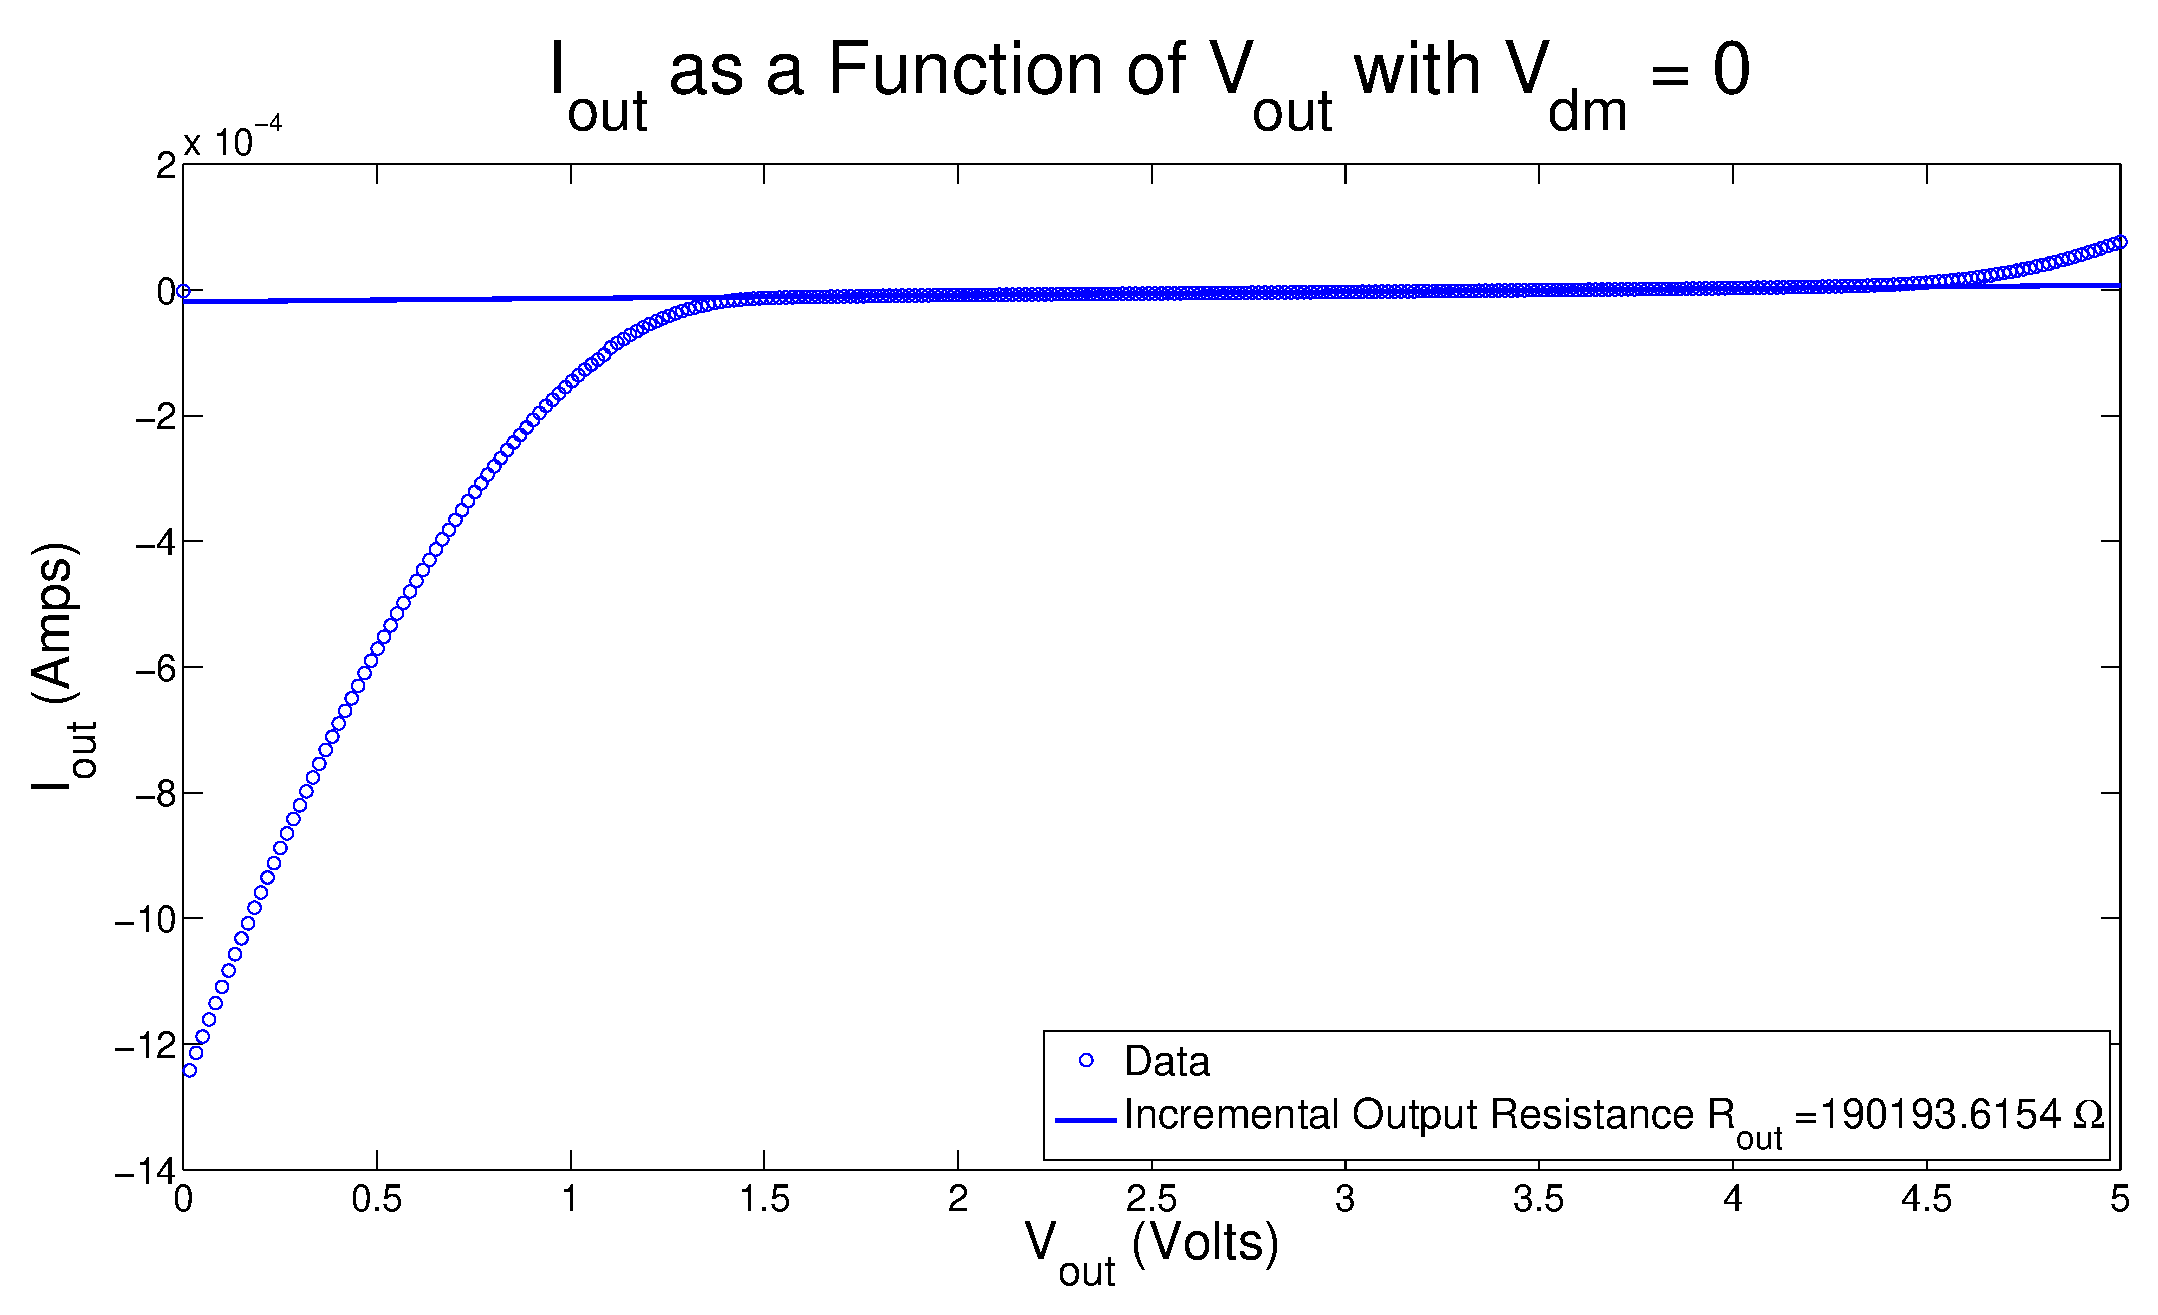
\includegraphics[width=\linewidth]{../Figures/Exp2P2.eps}
\caption{\Iout as a function of \Vout. The inverse of the slope of the shallow region of this graph is \Ro, the incremental resistance of the circuit. We extracted a value of 190193.615 $\Omega$ for \Ro, and used this to calculate \Adm in a separate manner than simply taking the slope of the vertical region in figure \ref{fig:exp2p1}}
\label{fig:exp2p2}
\end{figure}

We then fit a line to the steep linear region around $V_{dm} = \pm 0.005 V$, and used the slope to extract a value for \Adm. We fit to about 20 points along the line and found that $A_{dm} \approx 62.4146$. This large gain was theorized in the pre-lab (where we expected \Adm to be near infinite), but is not as large as expected. We expect \Vout to change drastically with \Vdm because the sign of \Vdm defines the flow of current, and opposite current flows likely cause large swings in \Vout. When $V_{dm} < 0$, $I_2 > I_1$, so \Vout lowers to allow more current through \Mfour, as \Mtwo pulls more current. Conversely, when $V_{dm} > 0$, $I_1 > I_2$, which causes \Vout to rise to prevent current flow through \Mfour, as \Mtwo cannot sink all of the current. We see the large swings in \Vout for small values of \Vdm as expected.

We next took the approach of calculating \Rout and \Gm, and multiplying these two properties of the circuit together in order to extract a different value for \Adm. Figure \ref{fig:exp2p3} shows \Iout as a function of \Vout, with an extracted slope that represents $\frac{1}{R_{out}}$. Figure \ref{fig:exp2p3} shows \Iout as a function of \Vdm, with an extracted value for \Gm. From these lines we found that $R_out = 190193.6154 \Omega$ and $G_m = 0.00044197 \Omega^{-1}$, which results in an extracted value for the differential mode gain of 84.0599. This is higher than the value we extracted from figure \ref{fig:exp2p1}, which could be due to compound error in the separate experiments or lines that don't exactly match the data they are fit to. Regardless, we see that \Adm is large, which is what we expect.

\begin{figure}[H]
\centering
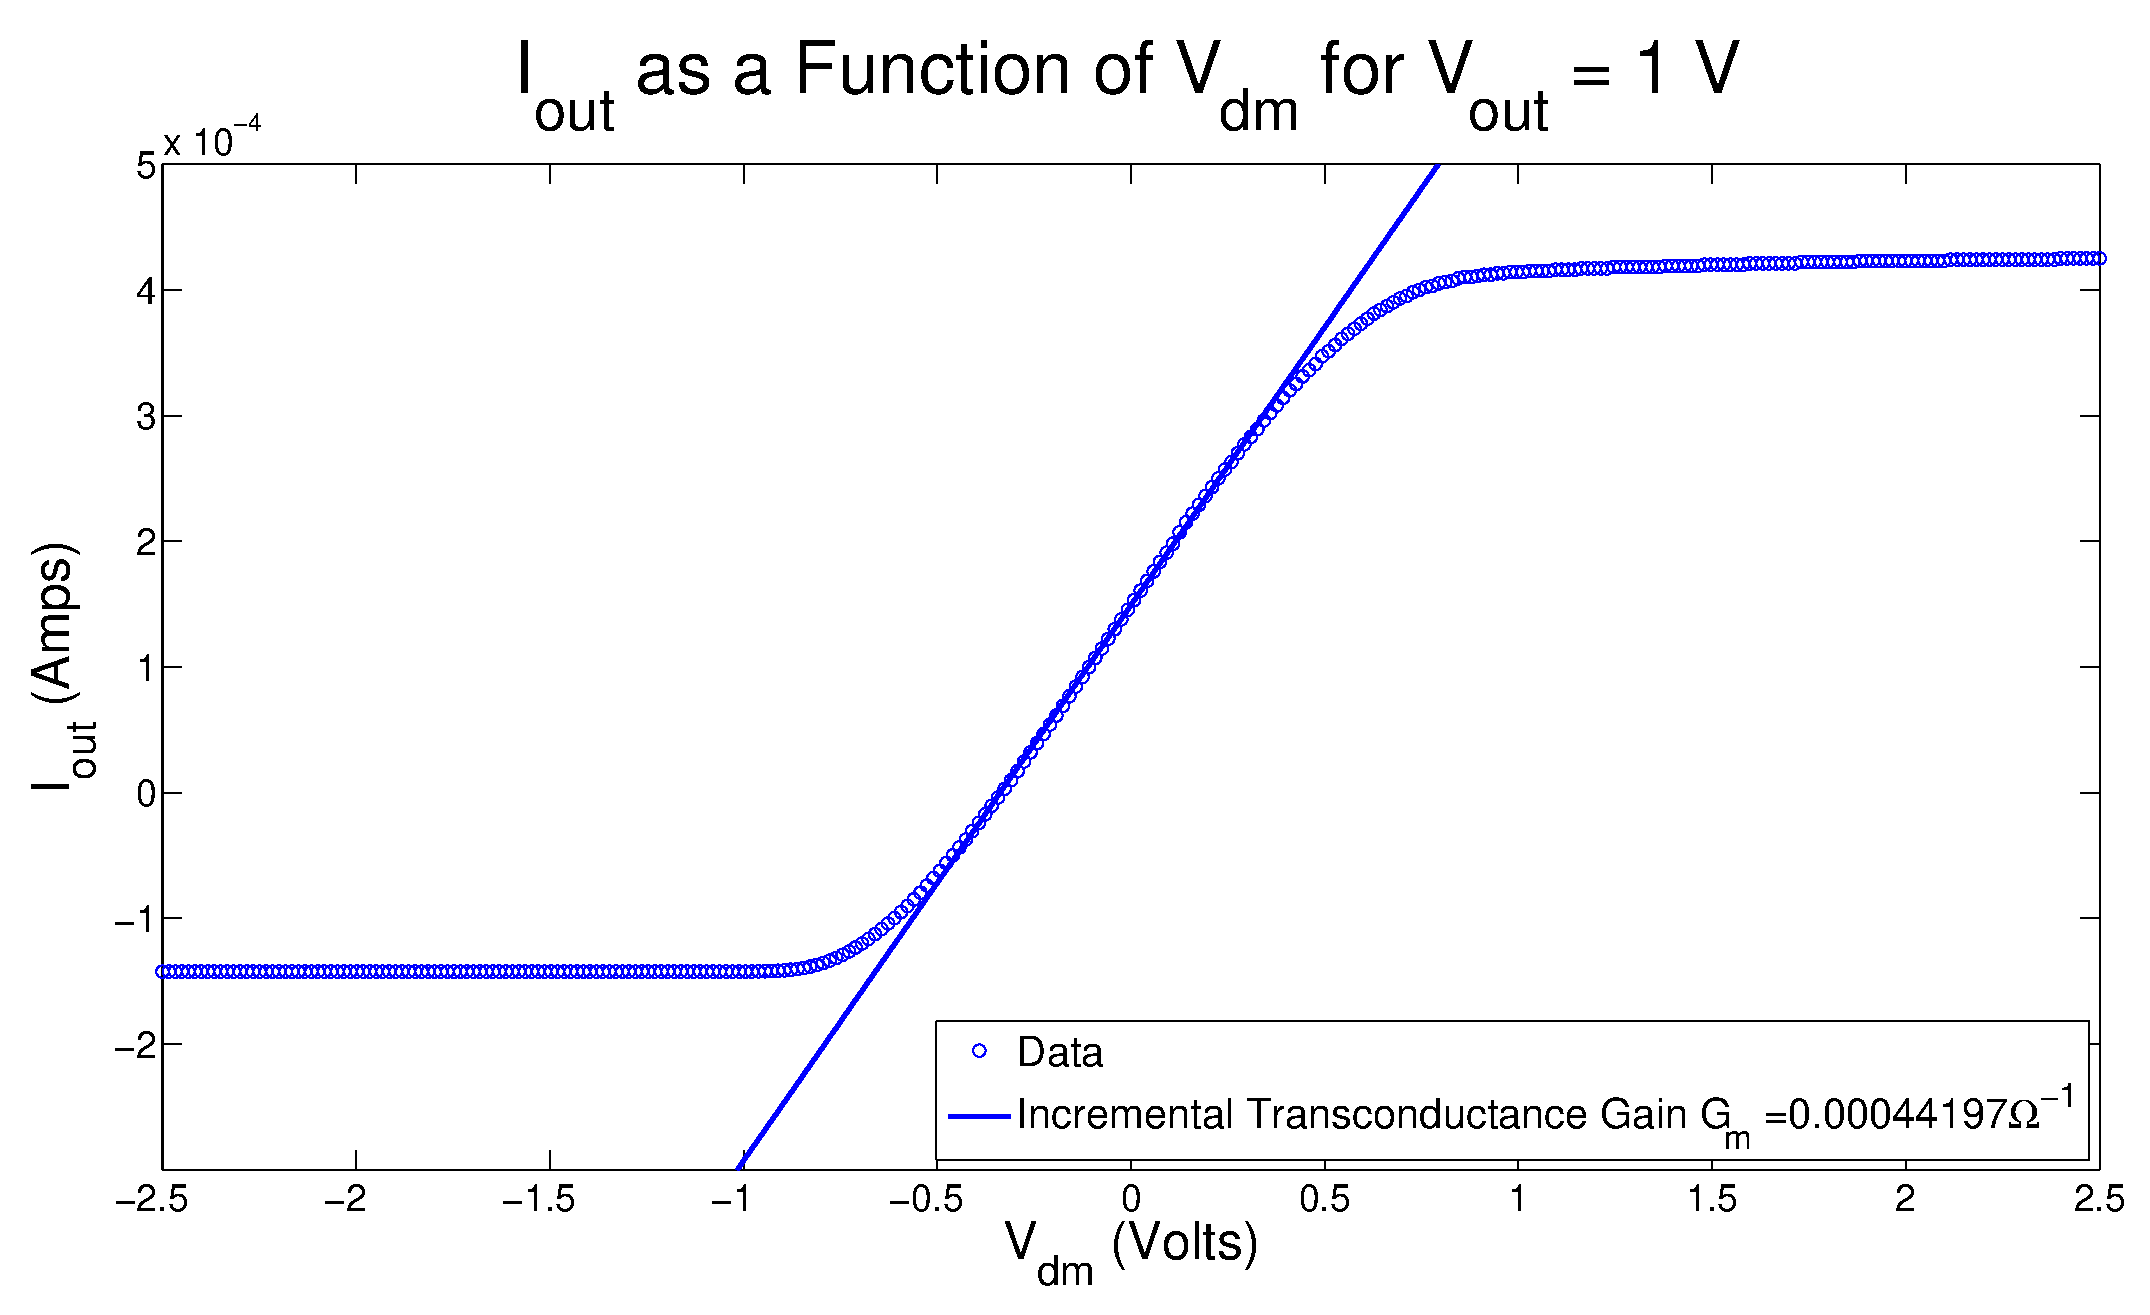
\includegraphics[width=\linewidth]{../Figures/Exp2P3.eps}
\caption{\Iout as a function of \Vdm. The slope of the linear region of this plot, around $|V_{out}| < 0.05 V$, can be used to extract \Gm, the incremental transconductance gain of this circuit. We extracted a value of 0.00044197 $\Omega^{-1}$ for \Gm, and used this value to calculate \Adm.}
\label{fig:exp2p3}
\end{figure}


An important attribute of a differential voltage amplifier is the Common-Mode-Rejection-Ratio, which we call the CMRR and is defined as:

\begin{equation}
CMRR = 20\textrm{log}_{10}(\frac{A_{dm}}{|A_{cm}|})
\end{equation}

For the value of \Adm derived from figure \ref{fig:exp2p1}, we found that the CMRR of this circuit is 49.7987, and for the \Adm value derived using figures \ref{fig:exp2p2} and \ref{fig:exp2p3}, the CMRR of this circuit is 52.3847. These two values for the CMRR are not very different, which indicates that the two different values of \Adm we calculated may not significantly affect the circuit behavior.

\section*{Experiment 3} 

\begin{figure}[H]
\centering
\includegraphics[width=0.5\linewidth]{../Figures/Voltage-follower}
\caption{Simple voltage follower we built in Experiment 3.}
\label{fig:voltagefollow}
\end{figure}

The last experiment we conducted involved connecting the inverting input of the differential amplifier, \Vtwo, to the output of the differential amplifier, \Vout. We expected the circuit to then behave like a unity-gain voltage follower, as seen in figure \ref{fig:voltagefollow}. In a unity-gain voltage follower, the output follows the non-inverting input, so we expect the ratio between \Vout and \Vin to be 1.

\begin{figure}[H]
\centering
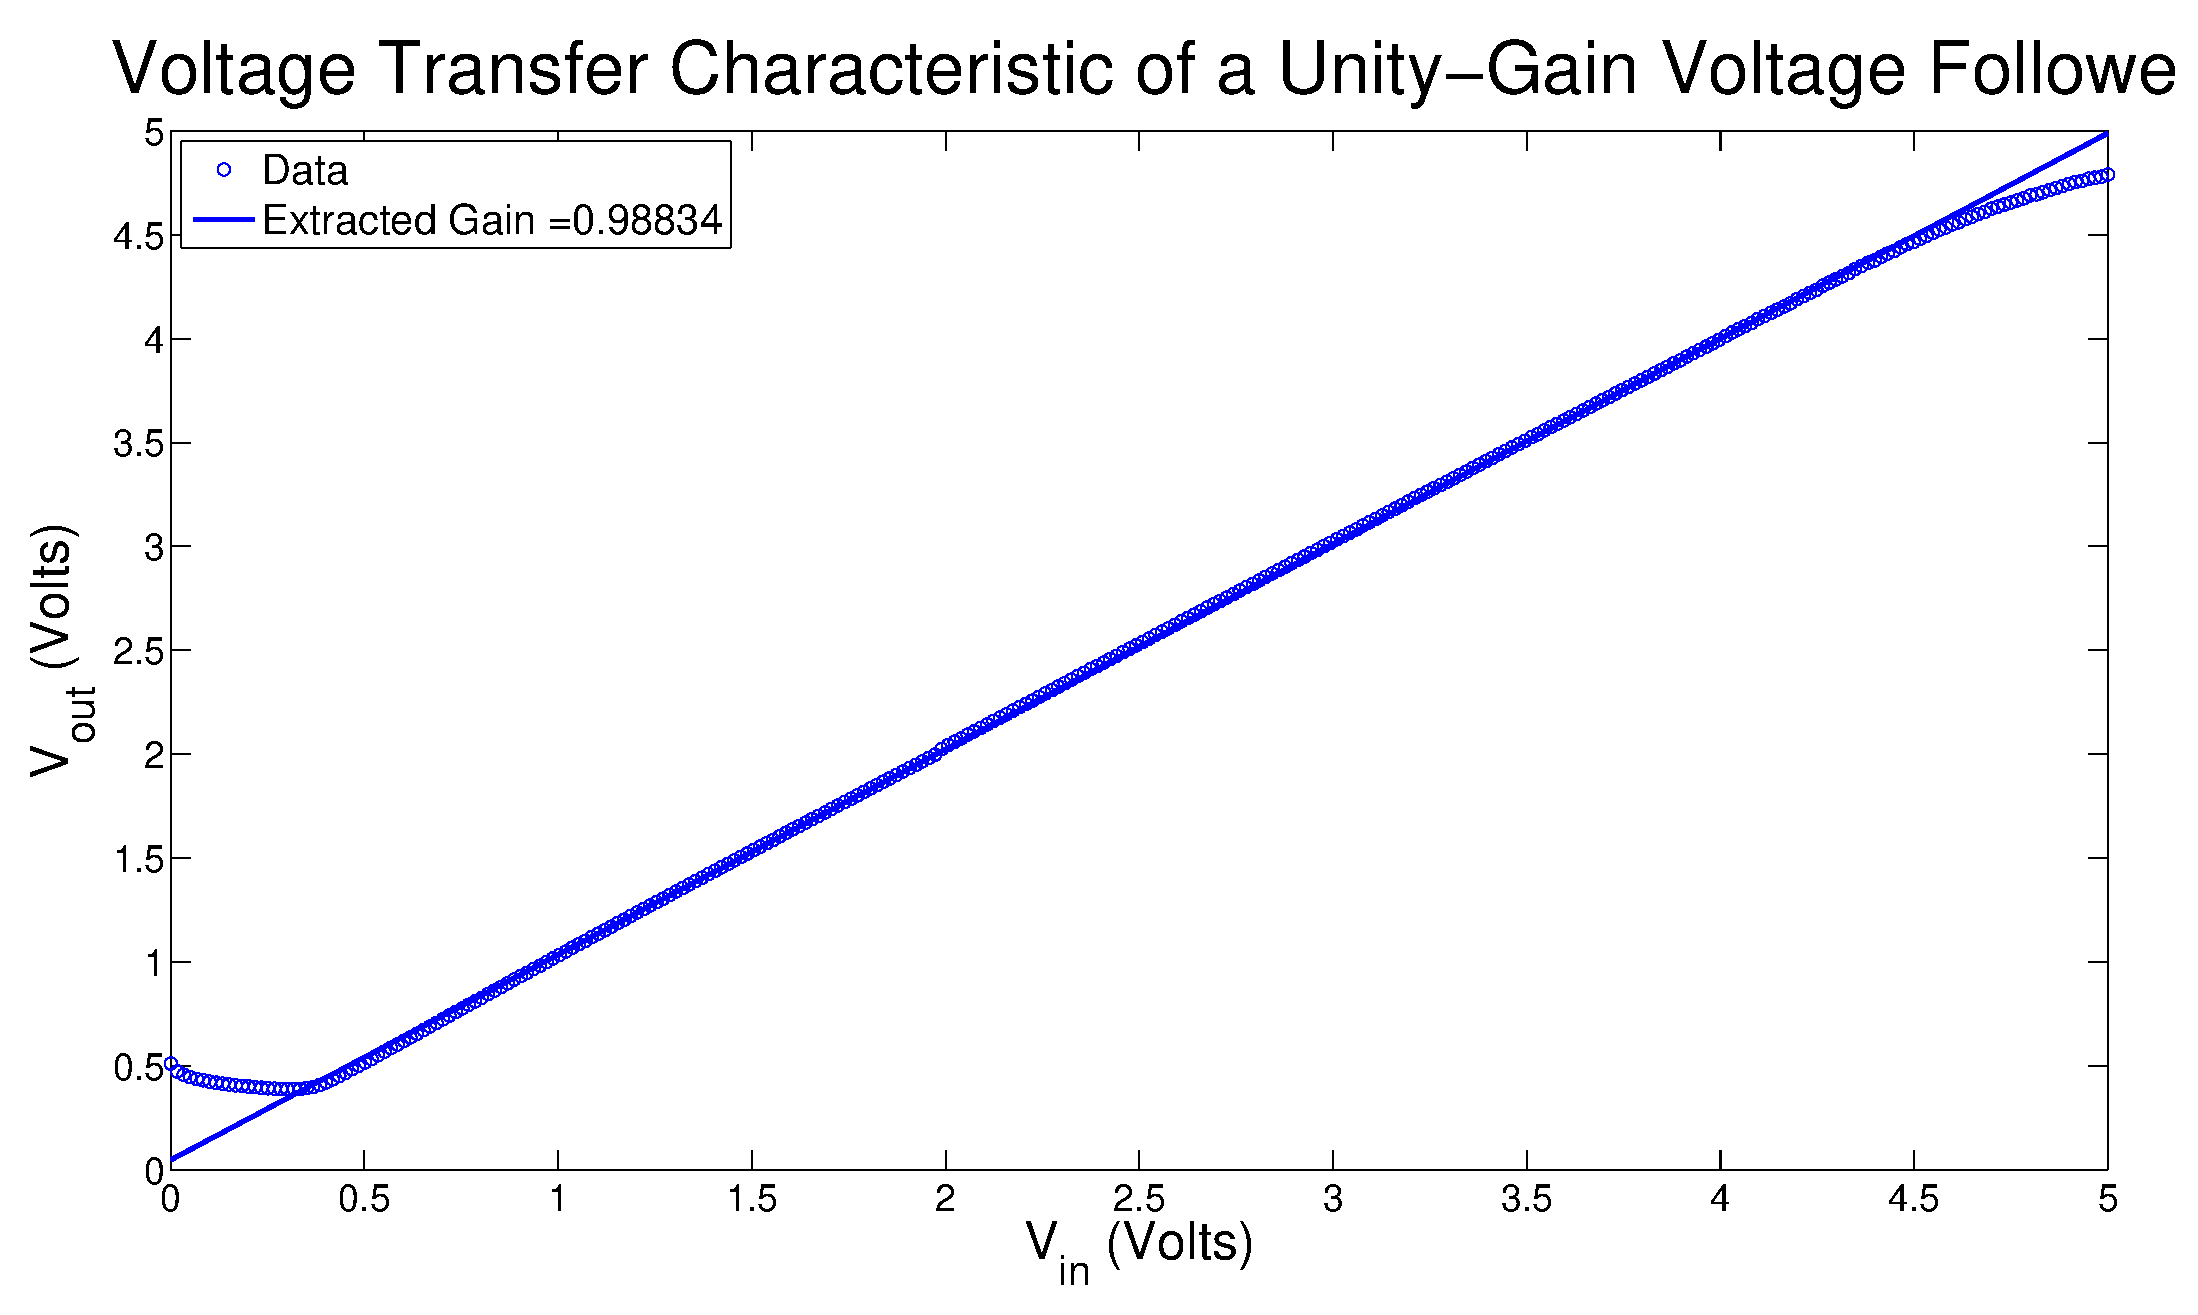
\includegraphics[width=\linewidth]{../Figures/Exp3P1.eps}
\caption{Something descriptive..}
\label{fig:exp3p1}
\end{figure}

So we connected the output and the input of the differential amplifier and measured \Vout as we swept \Vin from ground to \Vdd. The results are shown in figure \ref{fig:exp3p1}, in addition to a line fitted to the linear region of the voltage transfer characteristic. We extract the slope of this line and found that the actual gain of the follower was 0.98834, very close to the anticipated gain of 1. The slight deviation, a little over 1\%, can likely be attributed to experimental error. The behavior of the circuit for small values of \Vin can likely be attributed to both \Mone and \Mtwo operating in weak inversion, which causes \Iout to be the difference between their very small leakage currents, which therefore causes \Vout to change little for $0 \leq V_{in} \leq \approx 0.5 V.$

We can also see that the near-unity gain between \Vout and \Vin breaks down for values of \Vin near \Vdd. This could be due to the bias transistor not passing as much current as \Mone can pass, so as the gate voltage of \Mone increases, \Ib increases less than expected, which causes \Vout to increase less than linearly.

Since we expected $\frac{V_{out}}{V_{in}} \approx 1$, we next looked at the offset voltage of the bias transistor ($V_{out} - V_{in}$) in order to gain further insight into how our unity-gain buffer behaves compared to the ideal form of the circuit, which would have an offset voltage of 0.

\begin{figure}[H]
\centering
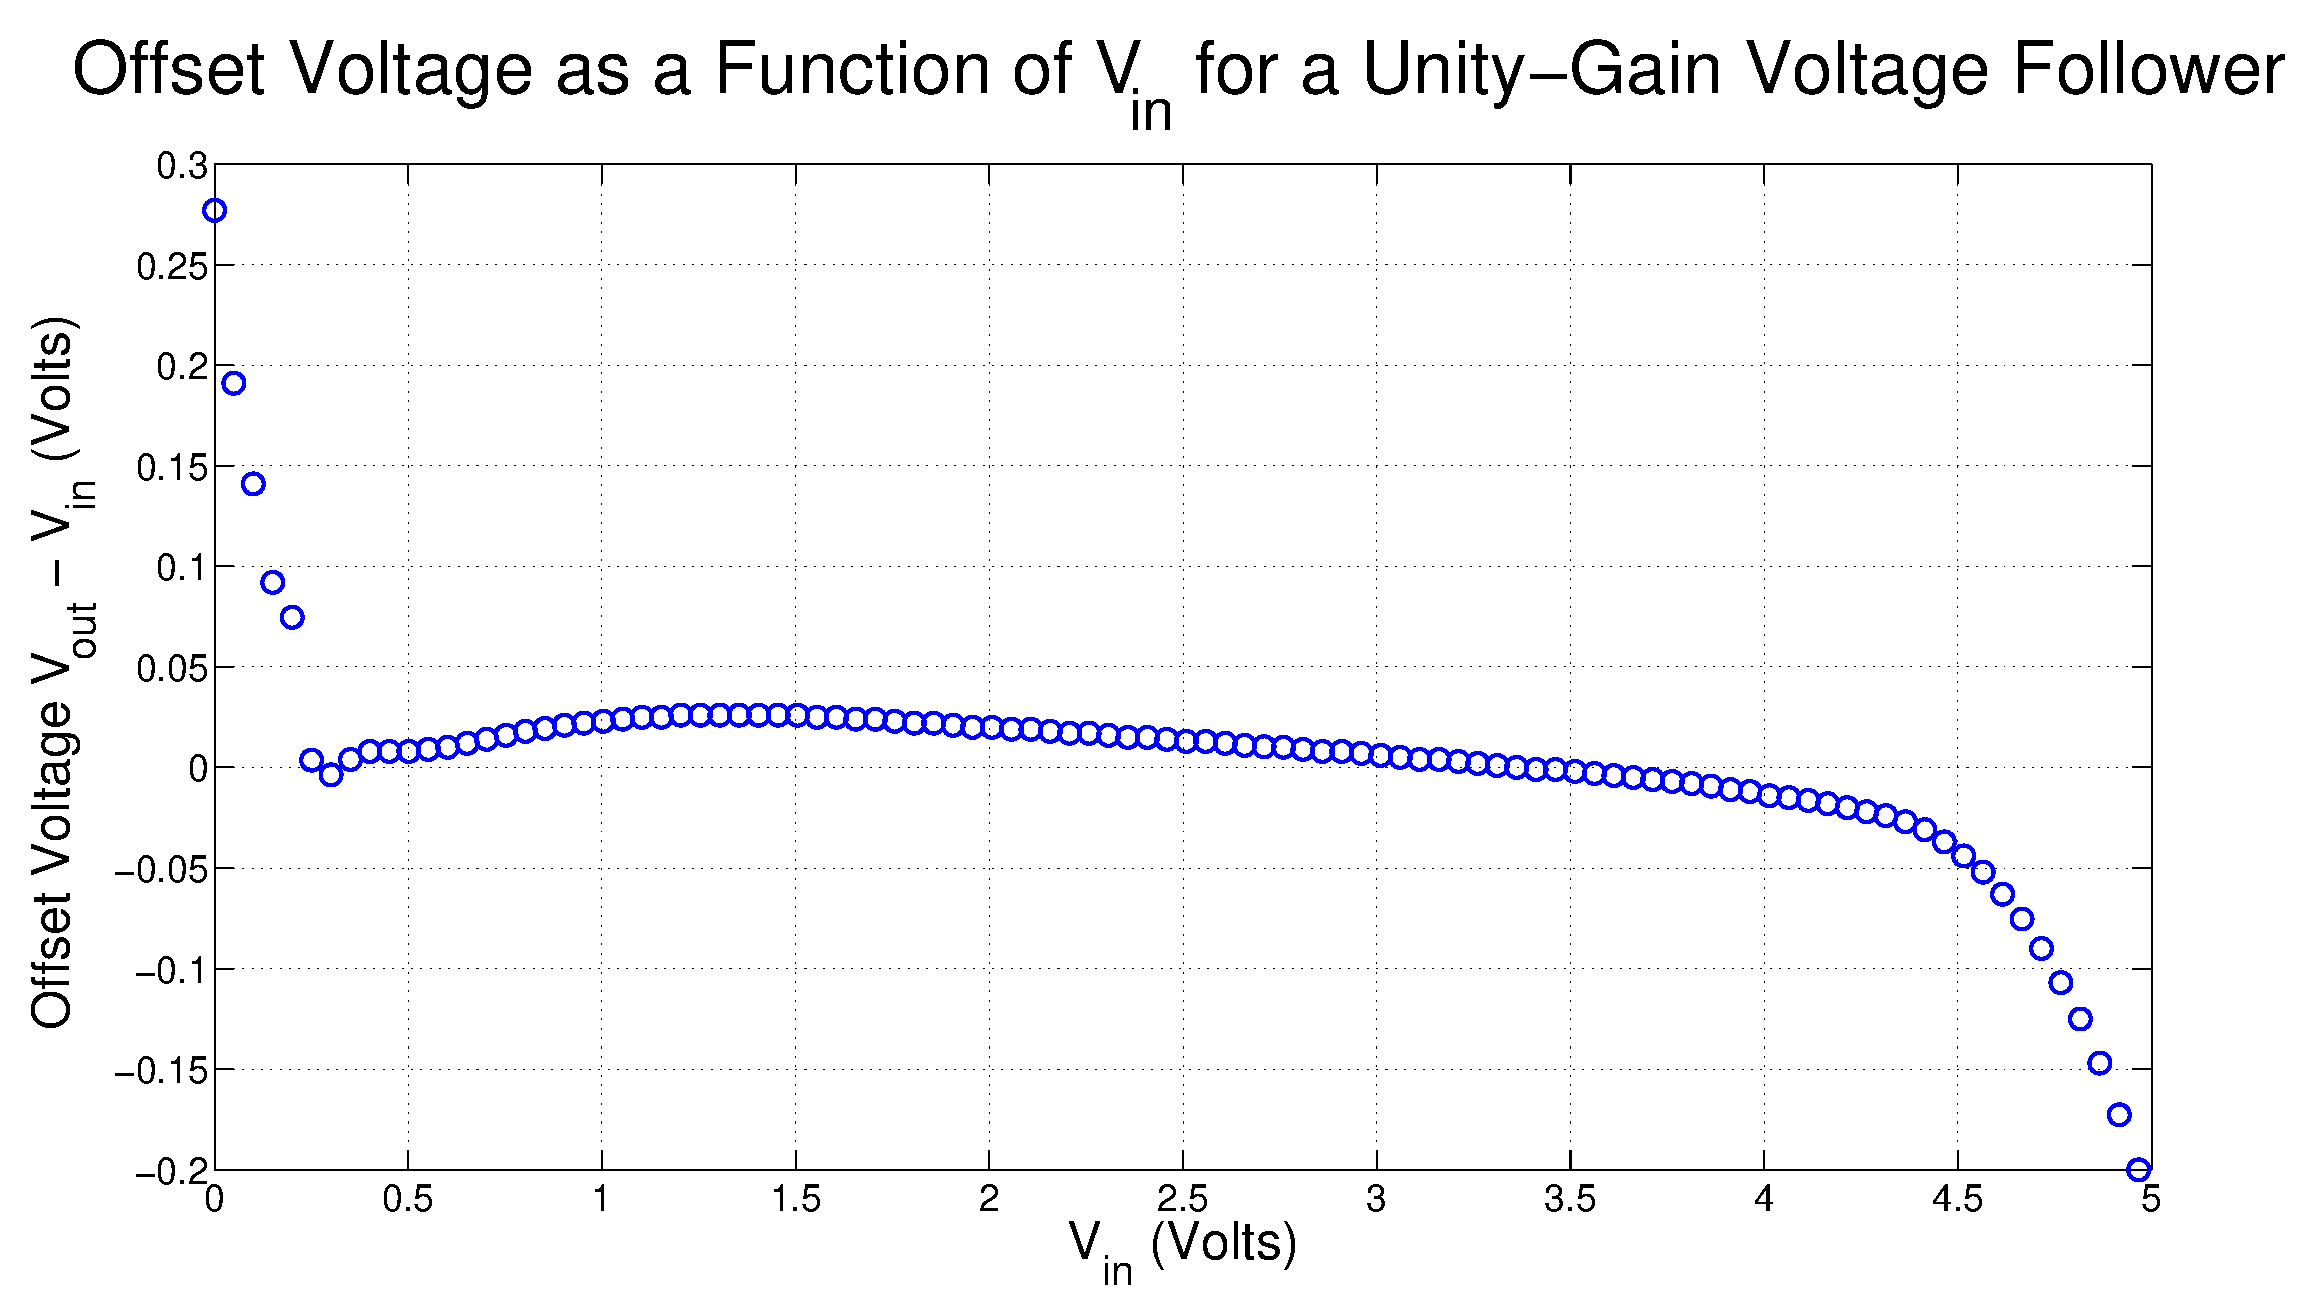
\includegraphics[width=\linewidth]{../Figures/Exp3P2.eps}
\caption{Something descriptive..}
\label{fig:exp3p2}
\end{figure}

Figure \ref{fig:exp2p2} shows the offset voltage of the buffer as a function of \Vin, and some interesting trends appear. We again see large deviations from the theoretical ideal at values of \Vin near ground and near \Vdd, which could be explained by leakage current and a saturated \Mb, respectively.

The trend in the middle of the data seems to take two forms: for $0.5 < V_{in} < 1.5$, the offset voltage has a small positive slope, but for $1.5 < V_{in} < 4.5$, this slope becomes negative, and the trend is far more linear. Generally, however, the offset voltage hovers around 0, and deviates by about $\pm 0.02 V$ throughout the region of linear operation that we saw in figure \ref{fig:exp3p1}. 


\end{document}